\chapter{Bases de Dados e Métodos de Geocodificação e Avaliação} \label{desenvolvimento}

Para avaliar a qualidade das APIs de geocodificação utilizadas no TerraLAB, recorremos a duas bases de dados padrão-ouro como referência. Utilizando essas bases, calculamos a medida de erro e conduzimos diversas métricas com base nessa medida.

\section{Bases de Dados}
Foram coletadas duas bases de dados distintas para este trabalho.

A primeira base coletada é proveniente do \href{https://centrodametropole.fflch.usp.br/pt-br}{Centro de Estudos da Metrópole (CEM)}. Essa base consiste em 12.502 endereços de escolas públicas e particulares do ensino básico da região metropolitana de São Paulo. A coleta desses dados foi realizada manualmente pelo CEM, utilizando GPS para registrar as coordenadas. Além das informações sobre os endereços, a base também contém uma variedade de informações sobre as escolas, possibilitando diversas análises relacionadas a esses dados. O CEM também disponibilizou um \href{http://200.144.244.241:3002/geolocation}{mapa de cluster} que exibe todas as escolas, facilitando a visualização da localização de cada uma delas e da densidade das escolas em São Paulo e região. A Figura \ref{fig:siteCEM} mostra o mapa de cluster. Nele, é possível visualizar a localização das escolas individualmente (ao dar zoom) e, ao dar zoom-out, a concentração de escolas em determinadas áreas, utilizando um sistema de cores no qual laranja representa muitas escolas, amarelo representa uma quantidade média e verde representa poucas escolas. 

\begin{figure} 
    \centering
    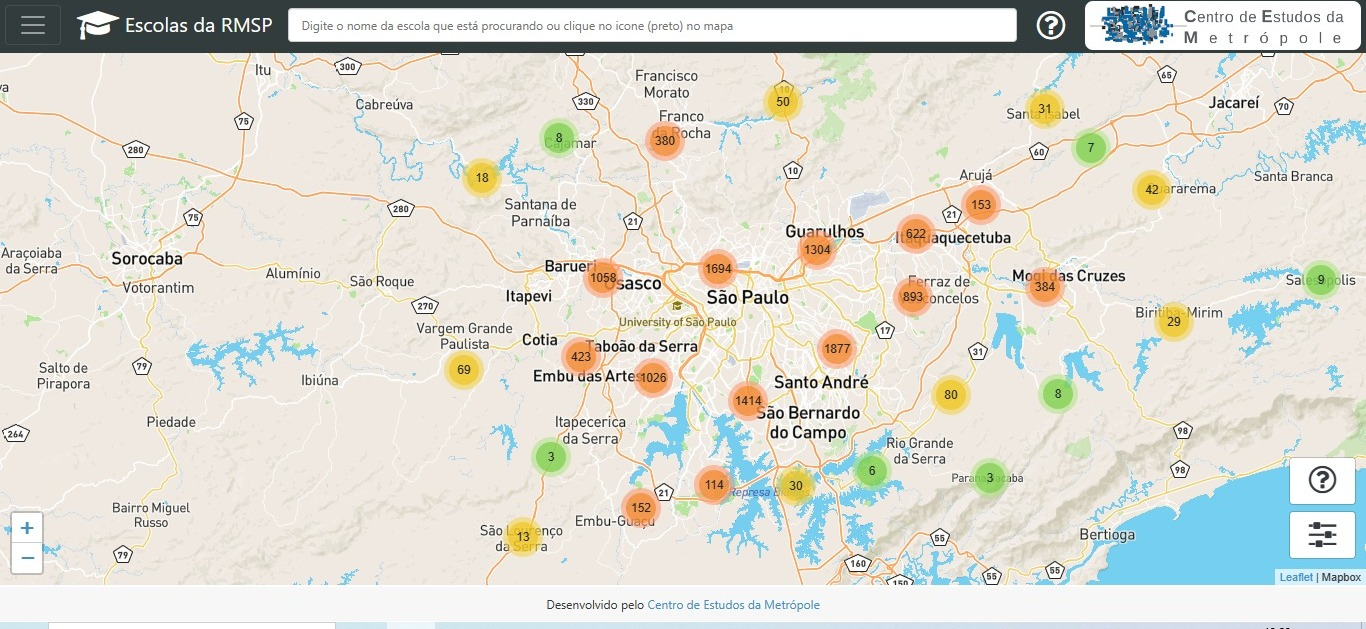
\includegraphics[width=0.8\textwidth]{Figuras/siteCEM.jpeg}
    \caption{Mapa de clusters do Centro de Estudos da Metrópole}
    \label{fig:siteCEM}
\end{figure}

A segunda base de dados coletada foi fornecida pela \cite{Prodabel}, a empresa de informática e informação da prefeitura de Belo Horizonte. A descoberta dessa base de dados foi possibilitada pelo artigo de referência \cite{Clodoveu2011}. Essa base de dados é mantida e atualizada mensalmente por 27 empresas, tanto públicas quanto privadas, de Belo Horizonte. Essas empresas têm a responsabilidade de relatar quaisquer inconsistências encontradas na base e de fornecer novos dados à medida que os adquirem. Ela é considerada uma fonte confiável de informações, pois está em constante atualização e é amplamente utilizada por diversos serviços da prefeitura. Um exemplo notável é o uso da base para georreferenciamento na distribuição de alunos da rede pública.

Na data de coleta, essa base continha um total de 763.229 endereços. A prefeitura disponibiliza um \href{https://bhmap.pbh.gov.br}{site com um mapa} que permite a visualização desses endereços. A Figura \ref{fig:siteProdabel} mostra esse site, e na barra de pesquisa, os usuários podem pesquisar endereços específicos e marcá-los no mapa. É importante notar que, ao contrário da maioria das APIs de geocodificação, todos os endereços foram posicionados em cima dos edifícios representados. A discrepância entre essa abordagem e a prática comum de colocar o endereço na frente do edifício pode causar um pequeno erro de alguns metros na comparação da geocodificação.

\begin{figure}
    \centering
    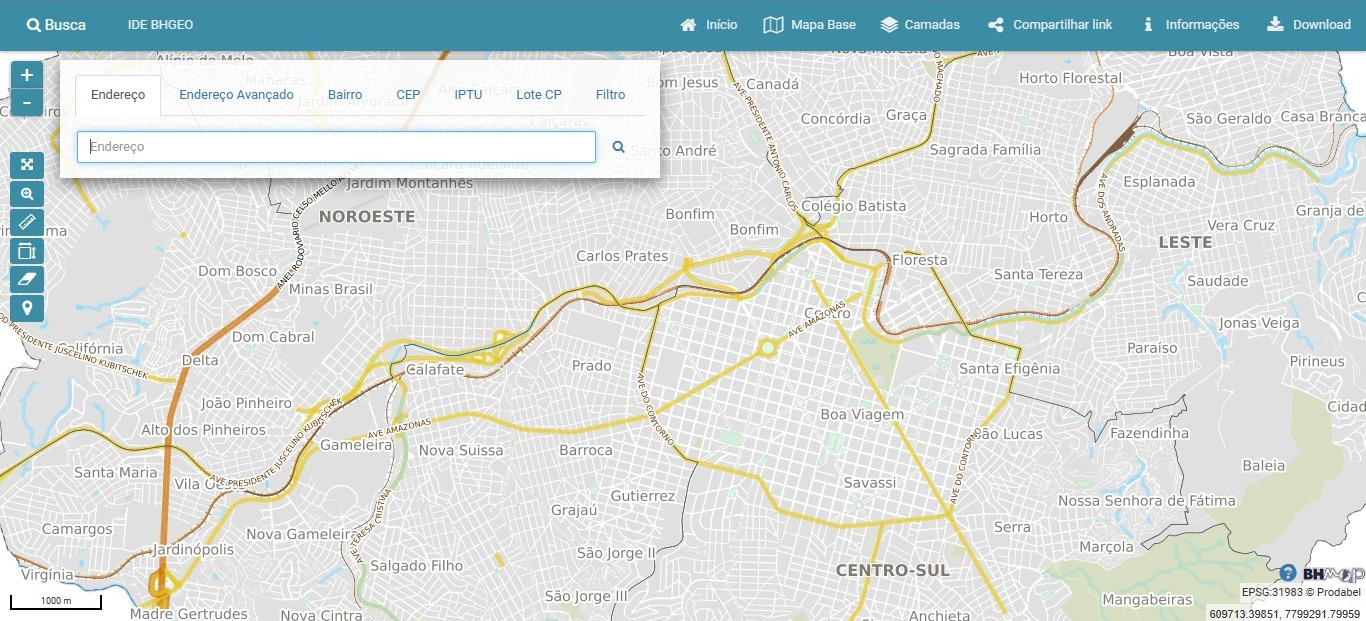
\includegraphics[width=0.8\textwidth]{Figuras/siteProdabel.jpeg}
    \caption{Site da Prodabel para pesquisa de endereços. }
    \label{fig:siteProdabel}
\end{figure}

Devido a limitações computacionais tanto dos autores deste trabalho quanto da aplicação responsável pela geocodificação, optamos por realizar uma amostragem da base de Belo Horizonte, com o intuito de reduzir a quantidade de dados processados. Nossa amostra consiste em 85.000 endereços da cidade. A fim de garantir uma distribuição uniforme dos endereços no espaço, empregamos o método do hipercubo latino para a amostragem. A Figura \ref{fig:baseBh} apresenta dois gráficos contendo os pontos da base original e os da amostra obtida. É possível observar que a amostra cobre toda a área abrangida. Além disso, verifica-se uma ligeira concentração nas regiões periféricas do desenho, permitindo uma melhor delimitação da cidade.

\begin{figure}[ht]
    \centering
    \begin{subfigure}[b]{0.45\textwidth}
      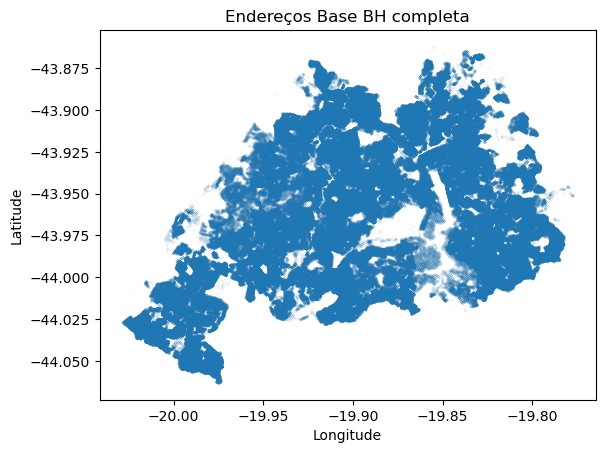
\includegraphics[width=\textwidth]{Figuras/baseBhToda.png}
      \caption{Completa}
      \label{fig:baseBhC}
    \end{subfigure}
    \hfill
    \begin{subfigure}[b]{0.45\textwidth}
      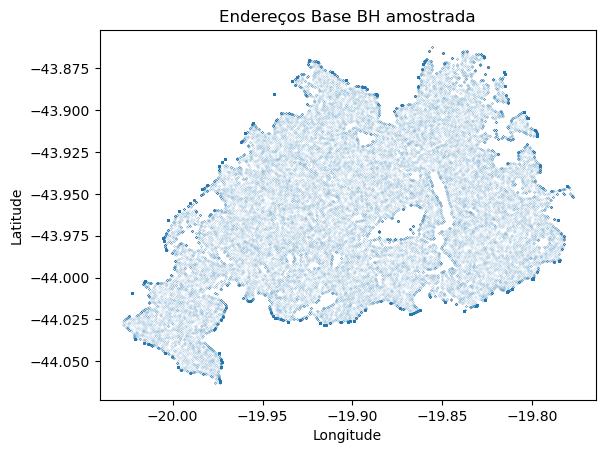
\includegraphics[width=\textwidth]{Figuras/baseBhAmostra.png}
      \caption{Amostra}
      \label{fig:baseBhA}
    \end{subfigure}
    \caption{Gráficos dos endereços da Base de Belo Horizonte e amostragem obtida}
    \label{fig:baseBh}
  \end{figure}


\section{Processo de Geocodificação}

\begin{figure}
    \centering
    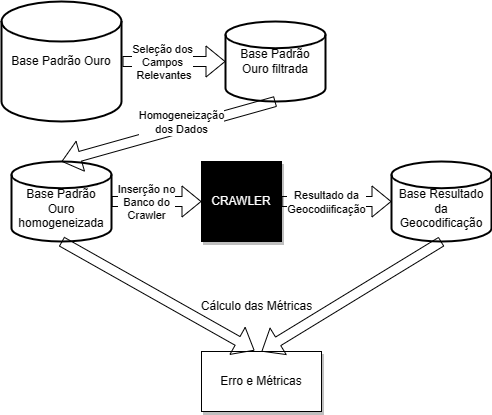
\includegraphics[width=0.8\textwidth]{Figuras/diagrama monografia.drawio.png}
    \caption{Esquematização do processo de preparação e geocodificação dos dados}
    \label{fig:diagramaMono}
\end{figure}
Após a coleta das bases, é necessário prepará-las para a geocodificação. A etapa de preparação de dados envolve a seleção dos campos relevantes da base de dados, como nome da rua, número, bairro, CEP e cidade. Em outras palavras, serão selecionados apenas os campos descritivos do endereço e os campos de localização geográfica do endereço. Após a seleção, os dados são homogeneizados, substituindo abreviações comuns por suas formas completas correspondentes. Esta etapa é conduzida pela equipe do TerraLAB e demonstrou-se que as APIs respondem de forma mais eficaz quando não há abreviações.

Para realizar a geocodificação, os endereços previamente preparados são inseridos no banco de dados do Crawler, a aplicação responsável por solicitar e coletar informações de geocodificação. Os endereços são então retirados do Crawler para serem geocodificados. É importante destacar que o processo de geocodificação é executado pela equipe de Back-end do TerraLAB, e, portanto, é considerado um processo de "caixa preta".

Após a conclusão da geocodificação, os endereços geocodificados, juntamente com suas coordenadas geográficas, são armazenados no mesmo banco de dados, mas em tabelas distintas. A Figura \ref{fig:diagramaMono} esquematiza todo esse processo essencial para o nosso trabalho.

\section{Método de Avaliação}

\subsection{Erro, Acurácia e Discrepância}

A principal métrica utilizada para avaliar a qualidade da geocodificação é o erro do endereço. Com base nesse erro, calcularemos medidas estatísticas, como a média, a mediana, o desvio padrão e a média aparada em 5\%, para analisar a precisão das GeoAPIs. Esse erro é calculado como a distância entre o ponto de referência e o ponto geocodificado pela GeoAPI, conforme a equação abaixo:

\begin{equation}
e = D(p_{\text{Ouro}}, p_{\text{Geo}})
\end{equation}

Onde:
\begin{itemize}
\item $e$ é o erro da geocodificação,
\item $D$ é uma função que calcula a distância em quilômetros,
\item $p_{\text{Ouro}}$ é o ponto da base Gold, e
\item $p_{\text{Geo}}$ é o ponto resultante da geocodificação.
\end{itemize}

Além disso, outra métrica utilizada é a taxa de resposta por API. Para alguns endereços da base de dados, as GeoAPIs podem retornar um erro, não fornecendo uma geocodificação válida. Nesse caso, nada é inserido no banco de dados. A taxa de resposta é calculada como a quantidade de endereços geocodificados dividida pela quantidade de endereços originais na base de dados. Esse valor é convertido em uma porcentagem para facilitar a compreensão dos resultados, de acordo com a seguinte fórmula:

\begin{equation}
\text{Taxa de Resposta (\%)} = \left(\frac{\text{Quantidade de Endereços Geocodificados}}{\text{Quantidade de Endereços Originais}}\right) \times 100\%
\end{equation}
